\documentclass[11pt,a4paper,]{article}
\usepackage{lmodern}

\usepackage{amssymb,amsmath}
\usepackage{ifxetex,ifluatex}
\usepackage{fixltx2e} % provides \textsubscript
\ifnum 0\ifxetex 1\fi\ifluatex 1\fi=0 % if pdftex
  \usepackage[T1]{fontenc}
  \usepackage[utf8]{inputenc}
\else % if luatex or xelatex
  \usepackage{unicode-math}
  \defaultfontfeatures{Ligatures=TeX,Scale=MatchLowercase}
\fi
% use upquote if available, for straight quotes in verbatim environments
\IfFileExists{upquote.sty}{\usepackage{upquote}}{}
% use microtype if available
\IfFileExists{microtype.sty}{%
\usepackage[]{microtype}
\UseMicrotypeSet[protrusion]{basicmath} % disable protrusion for tt fonts
}{}
\PassOptionsToPackage{hyphens}{url} % url is loaded by hyperref
\usepackage[unicode=true]{hyperref}
\hypersetup{
            pdftitle={Differences in CO2 emissions between countries on different basis},
            pdfborder={0 0 0},
            breaklinks=true}
\urlstyle{same}  % don't use monospace font for urls
\usepackage{geometry}
\geometry{a4paper, centering, text={16cm,24cm}}
\usepackage[style=authoryear-comp,]{biblatex}
\addbibresource{references.bib}
\usepackage{longtable,booktabs}
% Fix footnotes in tables (requires footnote package)
\IfFileExists{footnote.sty}{\usepackage{footnote}\makesavenoteenv{long table}}{}
\IfFileExists{parskip.sty}{%
\usepackage{parskip}
}{% else
\setlength{\parindent}{0pt}
\setlength{\parskip}{6pt plus 2pt minus 1pt}
}
\setlength{\emergencystretch}{3em}  % prevent overfull lines
\providecommand{\tightlist}{%
  \setlength{\itemsep}{0pt}\setlength{\parskip}{0pt}}
\setcounter{secnumdepth}{5}

% set default figure placement to htbp
\makeatletter
\def\fps@figure{htbp}
\makeatother


\title{Differences in CO2 emissions between countries on different basis}

%% MONASH STUFF

%% CAPTIONS
\RequirePackage{caption}
\DeclareCaptionStyle{italic}[justification=centering]
 {labelfont={bf},textfont={it},labelsep=colon}
\captionsetup[figure]{style=italic,format=hang,singlelinecheck=true}
\captionsetup[table]{style=italic,format=hang,singlelinecheck=true}


%% FONT
\RequirePackage{bera}
\RequirePackage[charter,expert,sfscaled]{mathdesign}
\RequirePackage{fontawesome}

%% HEADERS AND FOOTERS
\RequirePackage{fancyhdr}
\pagestyle{fancy}
\rfoot{\Large\sffamily\raisebox{-0.1cm}{\textbf{\thepage}}}
\makeatletter
\lhead{\textsf{\expandafter{\@title}}}
\makeatother
\rhead{}
\cfoot{}
\setlength{\headheight}{15pt}
\renewcommand{\headrulewidth}{0.4pt}
\renewcommand{\footrulewidth}{0.4pt}
\fancypagestyle{plain}{%
\fancyhf{} % clear all header and footer fields
\fancyfoot[C]{\sffamily\thepage} % except the center
\renewcommand{\headrulewidth}{0pt}
\renewcommand{\footrulewidth}{0pt}}

%% MATHS
\RequirePackage{bm,amsmath}
\allowdisplaybreaks

%% GRAPHICS
\RequirePackage{graphicx}
\setcounter{topnumber}{2}
\setcounter{bottomnumber}{2}
\setcounter{totalnumber}{4}
\renewcommand{\topfraction}{0.85}
\renewcommand{\bottomfraction}{0.85}
\renewcommand{\textfraction}{0.15}
\renewcommand{\floatpagefraction}{0.8}


%\RequirePackage[section]{placeins}

%% SECTION TITLES


%% SECTION TITLES (NEW: Changing sections and subsections color)
\RequirePackage[compact,sf,bf]{titlesec}
\titleformat*{\section}{\Large\sf\bfseries\color[rgb]{0.8, 0.7, 0.1 }}
\titleformat*{\subsection}{\large\sf\bfseries\color[rgb]{0.8, 0.7, 0.1 }}
\titleformat*{\subsubsection}{\sf\bfseries\color[rgb]{0.8, 0.7, 0.1 }}
\titlespacing{\section}{0pt}{2ex}{.5ex}
\titlespacing{\subsection}{0pt}{1.5ex}{0ex}
\titlespacing{\subsubsection}{0pt}{.5ex}{0ex}


%% TITLE PAGE
\def\Date{\number\day}
\def\Month{\ifcase\month\or
 January\or February\or March\or April\or May\or June\or
 July\or August\or September\or October\or November\or December\fi}
\def\Year{\number\year}

%% LINE AND PAGE BREAKING
\sloppy
\clubpenalty = 10000
\widowpenalty = 10000
\brokenpenalty = 10000
\RequirePackage{microtype}

%% PARAGRAPH BREAKS
\setlength{\parskip}{1.4ex}
\setlength{\parindent}{0em}

%% HYPERLINKS
\RequirePackage{xcolor} % Needed for links
\definecolor{darkblue}{rgb}{0,0,.6}
\RequirePackage{url}

\makeatletter
\@ifpackageloaded{hyperref}{}{\RequirePackage{hyperref}}
\makeatother
\hypersetup{
     citecolor=0 0 0,
     breaklinks=true,
     bookmarksopen=true,
     bookmarksnumbered=true,
     linkcolor=darkblue,
     urlcolor=blue,
     citecolor=darkblue,
     colorlinks=true}

\usepackage[showonlyrefs]{mathtools}
\usepackage[no-weekday]{eukdate}

%% BIBLIOGRAPHY

\makeatletter
\@ifpackageloaded{biblatex}{}{\usepackage[style=authoryear-comp, backend=biber, natbib=true]{biblatex}}
\makeatother
\ExecuteBibliographyOptions{bibencoding=utf8,minnames=1,maxnames=3, maxbibnames=99,dashed=false,terseinits=true,giveninits=true,uniquename=false,uniquelist=false,doi=false, isbn=false,url=true,sortcites=false}

\DeclareFieldFormat{url}{\texttt{\url{#1}}}
\DeclareFieldFormat[article]{pages}{#1}
\DeclareFieldFormat[inproceedings]{pages}{\lowercase{pp.}#1}
\DeclareFieldFormat[incollection]{pages}{\lowercase{pp.}#1}
\DeclareFieldFormat[article]{volume}{\mkbibbold{#1}}
\DeclareFieldFormat[article]{number}{\mkbibparens{#1}}
\DeclareFieldFormat[article]{title}{\MakeCapital{#1}}
\DeclareFieldFormat[article]{url}{}
%\DeclareFieldFormat[book]{url}{}
%\DeclareFieldFormat[inbook]{url}{}
%\DeclareFieldFormat[incollection]{url}{}
%\DeclareFieldFormat[inproceedings]{url}{}
\DeclareFieldFormat[inproceedings]{title}{#1}
\DeclareFieldFormat{shorthandwidth}{#1}
%\DeclareFieldFormat{extrayear}{}
% No dot before number of articles
\usepackage{xpatch}
\xpatchbibmacro{volume+number+eid}{\setunit*{\adddot}}{}{}{}
% Remove In: for an article.
\renewbibmacro{in:}{%
  \ifentrytype{article}{}{%
  \printtext{\bibstring{in}\intitlepunct}}}

\AtEveryBibitem{\clearfield{month}}
\AtEveryCitekey{\clearfield{month}}

\makeatletter
\DeclareDelimFormat[cbx@textcite]{nameyeardelim}{\addspace}
\makeatother

\author{\sf\Large\textbf{ Ishita Khanna}\\ {\sf\large Student\\[0.5cm]} \sf\Large\textbf{ Wanxin Chen}\\ {\sf\large Student\\[0.5cm]} \sf\Large\textbf{ Gui Gao}\\ {\sf\large Student\\[0.5cm]} \sf\Large\textbf{ Shu Wang}\\ {\sf\large Student\\[0.5cm]}}

\date{\sf\Date~\Month~\Year}
\makeatletter
\lfoot{\sf Khanna, Chen, Gao, Wang: \@date}
\makeatother


%%%% PAGE STYLE FOR FRONT PAGE OF REPORTS

\makeatletter
\def\organization#1{\gdef\@organization{#1}}
\def\telephone#1{\gdef\@telephone{#1}}
\def\email#1{\gdef\@email{#1}}
\makeatother
  \organization{Australian Government COVID19}

  \def\name{Our consultancy \newline add names \&\newline add names}

  \telephone{(03) 9905 2478}

  \email{questions@company.com}                 %NEW: New email addresss

\def\webaddress{\url{http://company.com/stats/consulting/}} %NEW: URl
\def\abn{12 377 614 630}                                    % NEW: ABN
\def\logo{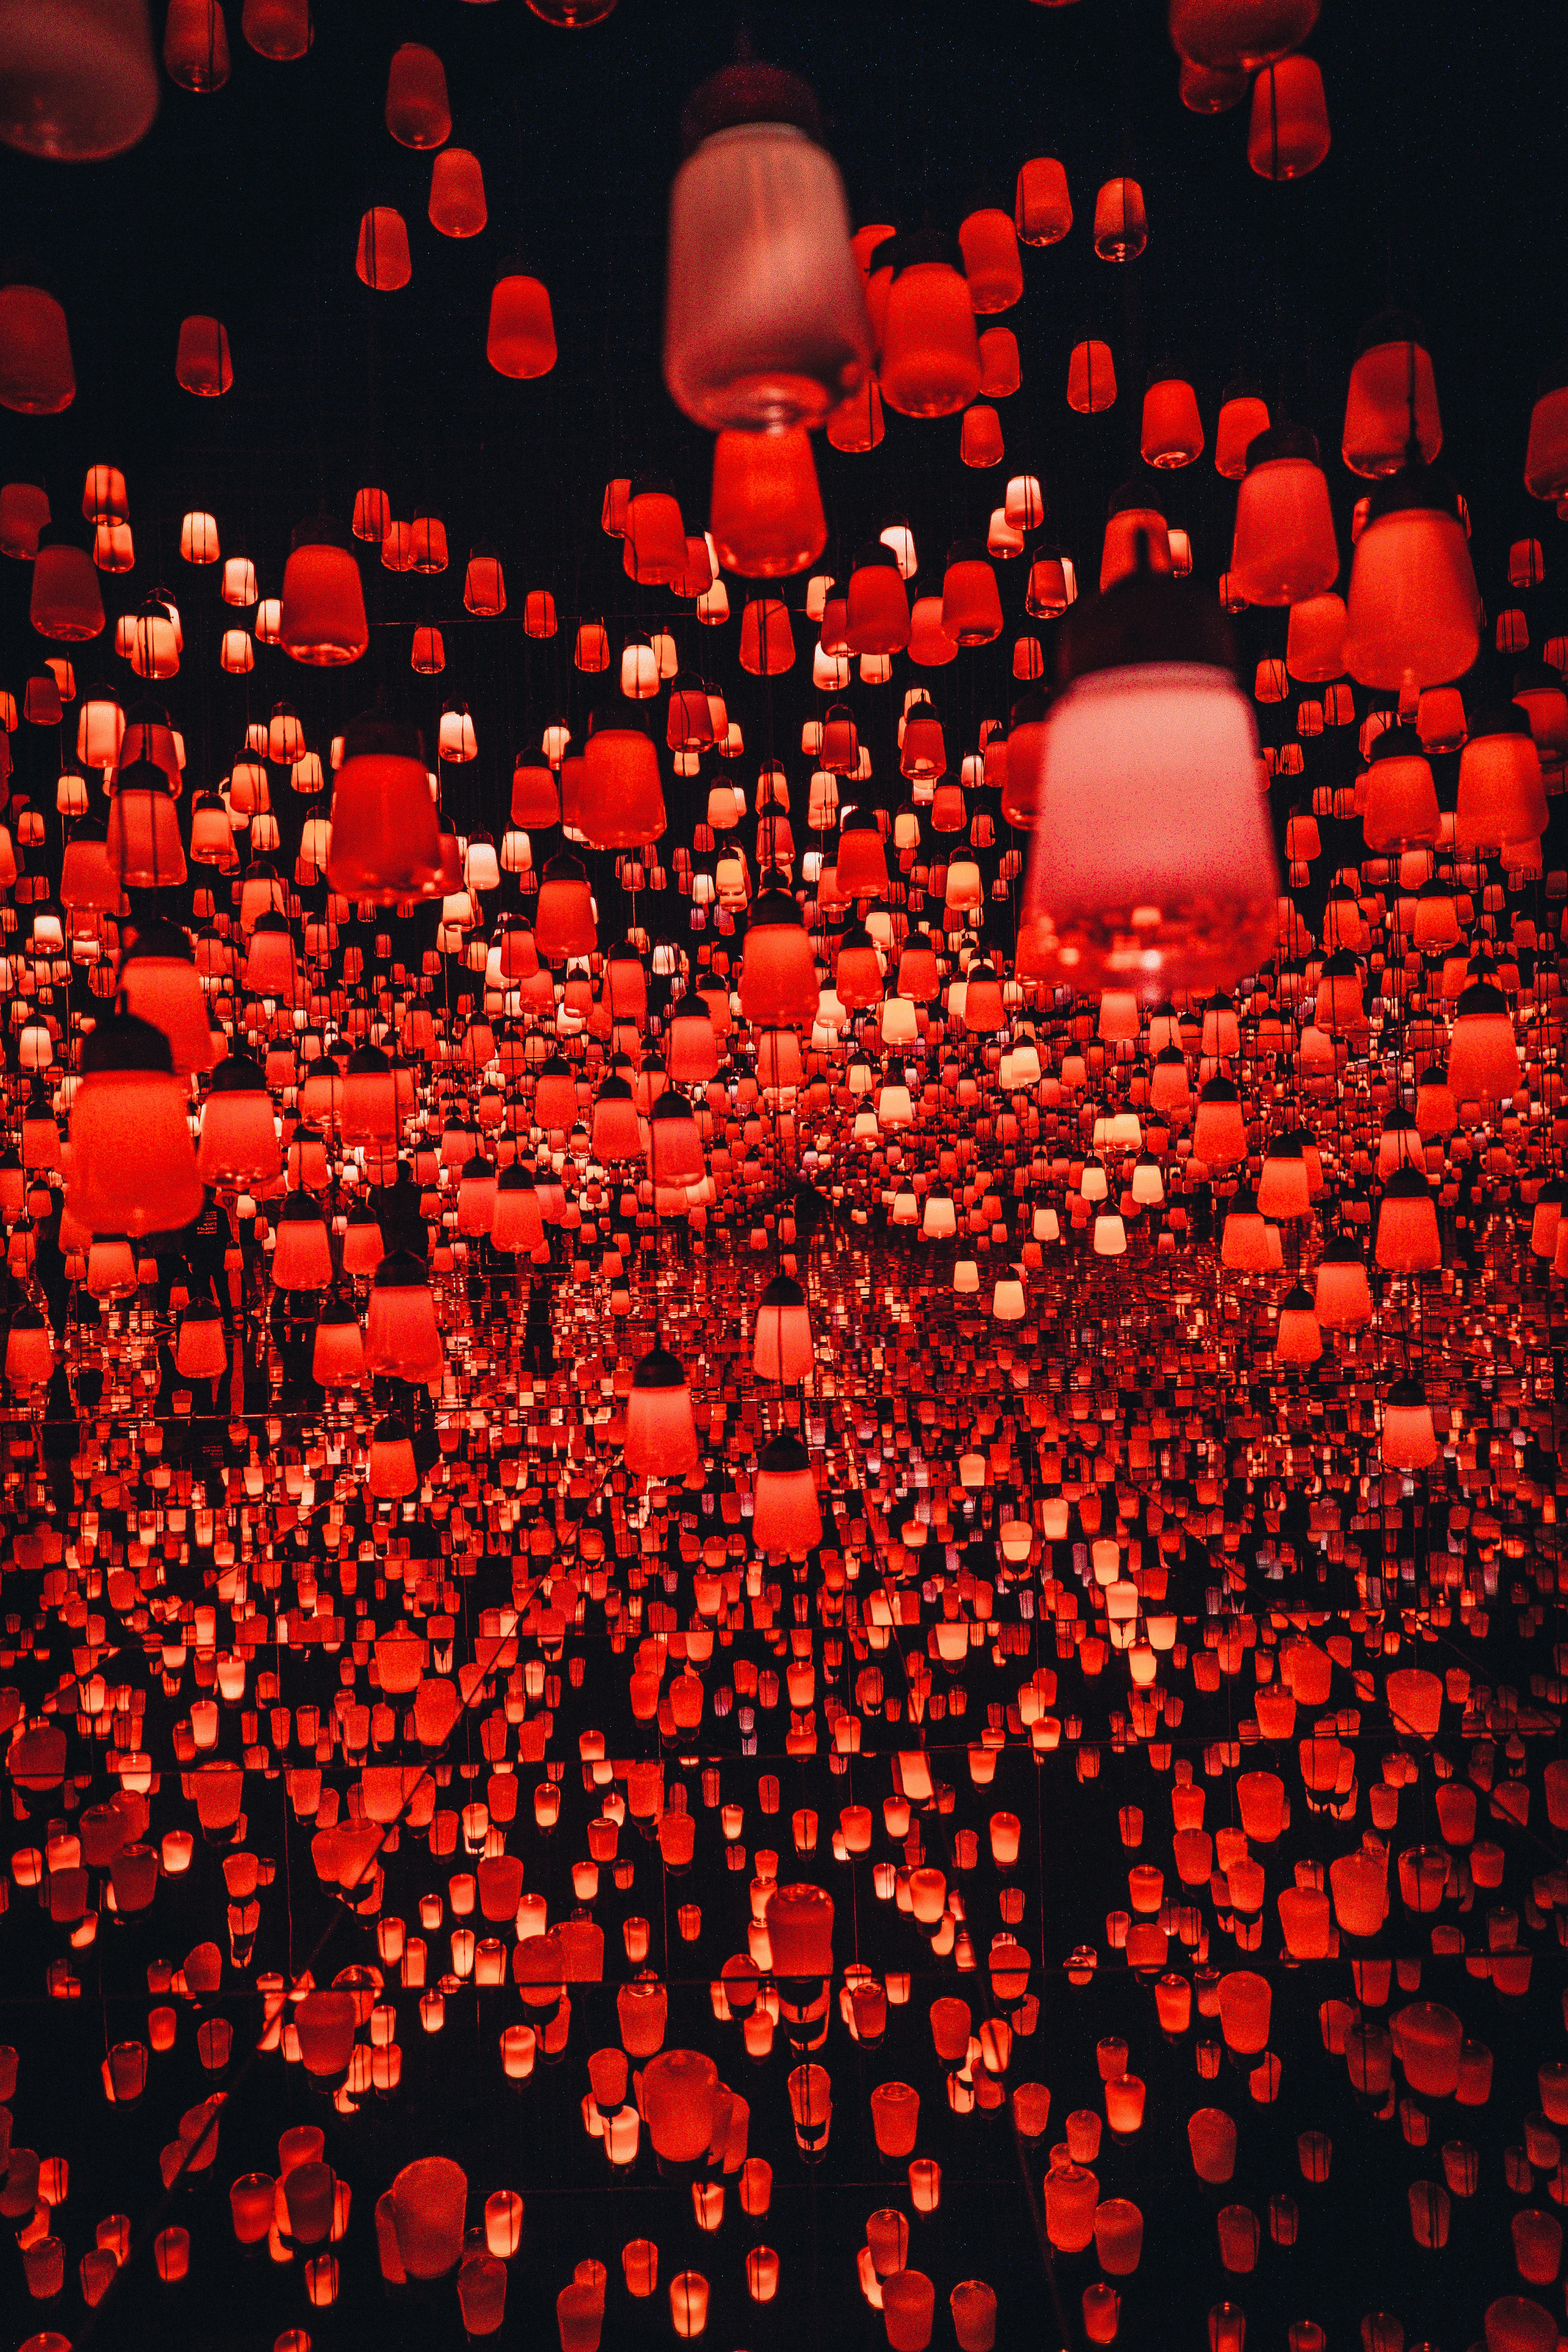
\includegraphics[width=6cm]{Figures/logo}}  %NEW: Changing logo
\def\extraspace{\vspace*{1.6cm}}
\makeatletter
\def\contactdetails{\faicon{phone} & \@telephone \\
                    \faicon{envelope} & \@email}
\makeatother

%%%% FRONT PAGE OF REPORTS

\def\reporttype{Report for}

\long\def\front#1#2#3{
\newpage
\begin{singlespacing}
\thispagestyle{empty}
\vspace*{-1.4cm}
\hspace*{-1.4cm}
\hbox to 16cm{
  \hbox to 6.5cm{\vbox to 14cm{\vbox to 25cm{
    \logo
    \vfill
    \parbox{6.3cm}{\raggedright
      \sf\color[rgb]{0.8, 0.7, 0.1 }    % NEW color 
      {\large\textbf{\name}}\par
      \vspace{.7cm}
      \tabcolsep=0.12cm\sf\small
      \begin{tabular}{@{}ll@{}}\contactdetails
      \end{tabular}
      \vspace*{0.3cm}\par
      ABN: \abn\par
    }
  }\vss}\hss}
  \hspace*{0.2cm}
  \hbox to 1cm{\vbox to 14cm{\rule{4pt}{26.8cm}\vss}\hss\hfill}  %NEW: Thicker line
  \hbox to 10cm{\vbox to 14cm{\vbox to 25cm{   
      \vspace*{3cm}\sf\raggedright
      \parbox{11cm}{\sf\raggedright\baselineskip=1.2cm
         \fontsize{24.88}{30}\color[rgb]{0, 0.29, 0.55}\sf\textbf{#1}}   % NEW: title color blue
      \par
      \vfill
      \large
      \vbox{\parskip=0.8cm #2}\par
      \vspace*{2cm}\par
      \reporttype\\[0.3cm]
      \hbox{#3}%\\[2cm]\
      \vspace*{1cm}
      {\large\sf\textbf{\Date~\Month~\Year}}
   }\vss}
  }}
\end{singlespacing}
\newpage
}

\makeatletter
\def\titlepage{\front{\expandafter{\@title}}{\@author}{\@organization}}
\makeatother

\usepackage{setspace}
\setstretch{1.5}

%% Any special functions or other packages can be loaded here.
\usepackage{booktabs}
\usepackage{longtable}
\usepackage{array}
\usepackage{multirow}
\usepackage{wrapfig}
\usepackage{float}
\usepackage{colortbl}
\usepackage{pdflscape}
\usepackage{tabu}
\usepackage{threeparttable}
\usepackage{threeparttablex}
\usepackage[normalem]{ulem}
\usepackage{makecell}
\usepackage{xcolor}


\begin{document}
\titlepage

\hypertarget{introduction}{%
\section{Introduction}\label{introduction}}

Carbon dioxide emissions are a major driver of global climate change. It is widely accepted that in order to avoid the worst effects of climate change, the world needs to reduce emissions as a matter of urgency. It is believed that most environmental pollution is associated with developed countries; The recent occurrence of abnormal natural phenomena such as fires in Australia demonstrates the profound impact of excessive carbon emissions on the climate.however, recent studies have shown the role that developing countries play in contributing to climate change.

\section*{Country "India" and "Sri Lanka"}

\hypertarget{research-question}{%
\section{Research Question}\label{research-question}}

1.Comparing both the countries based on population and Energy\_use\_kg\_of\_oil\_equivalent\_per\_capita from 1970 to 2013.

2.Analyzing data of India and Sri-Lanka based on the CO2 emission from 1970 to 2013.

\begin{table}[!h]

\caption{\label{tab:EnergyComparison}Total energy consumption in India and Sri Lanka}
\centering
\begin{tabular}[t]{lrr}
\toprule
Country\_Name & Total\_population & Total\_energy\\
\midrule
India & 5390725723 & 8378.171\\
Sri Lanka & 69624742 & 8086.842\\
\bottomrule
\end{tabular}
\end{table}

\begin{figure}[H]

{\centering \includegraphics[width=0.9\linewidth]{report_files/figure-latex/fig1-1} 

}

\caption{Release of CO2}\label{fig:fig1}
\end{figure}

\hypertarget{data-explanation}{%
\section{Data explanation}\label{data-explanation}}

\begin{itemize}
\tightlist
\item
  This is a data-set containing all the countries data having CO2 Emissions and urban population and energy usage as variables in different years from 1960 to 2018.
\item
  I then filtered the data based on two countries that I have to do comparison on i.e India and Sri Lanka while removing the null values from it using the \emph{na.omit} function.
\item
  Tried to analyze the data based on energy usage using \emph{kable} function.
\item
  Analyze he data based on CO2 Emission using \emph{ggplot} function with \emph{geom\_point} and \emph{geom\_line}.
\item
  It seems like there has been an increase in CO2 emission with the increase in time.
\end{itemize}

\hypertarget{referencing}{%
\section{Referencing}\label{referencing}}

Table \ref{tab:EnergyComparison} shows the comparison of India and Sri Lanka based on population and Energy usage in those area in different years.In figure \ref{fig:fig1}, I made graphical representation of Co2 emission in India and Sri Lanka in different time frame using line and scatter points graph.

\section*{Country "Andorra" and "Algeria"}

\hypertarget{research-question-1}{%
\section{Research Question}\label{research-question-1}}

\begin{enumerate}
\def\labelenumi{\arabic{enumi}.}
\item
  Analysis of the relationship between emissions generated by countries in different regions and income, based on data from Andorra and Algeria in 2010-2014.
\item
  Analysis of the relationship between emissions generated by countries in different regions and population , based on data from Andorra and Algeria in 2010-2014.
\end{enumerate}

\begin{table}[!h]

\caption{\label{tab:table-1}Cumulative CO2 emissions}
\centering
\begin{tabular}[t]{lr}
\toprule
Country\_Name & Total\_emissions\\
\midrule
\cellcolor{gray!6}{Algeria} & \cellcolor{gray!6}{17.35632}\\
Andorra & 29.64157\\
\bottomrule
\end{tabular}
\end{table}

\begin{figure}[H]

{\centering \includegraphics[width=0.75\linewidth]{report_files/figure-latex/fig-1-1} 

}

\caption{CO2 emissions}\label{fig:fig-1}
\end{figure}

\hypertarget{data-explanation-1}{%
\section{Data Explanation}\label{data-explanation-1}}

The trend of CO2 emissions per capita in Andorra, a developed country, is decreasing, which is in line with the EKC hypothesis mentioned, and developed countries will adopt environmental protection policies(\textcite{RE1}), but in terms of cumulative CO2 emissions, developed countries' emissions are still higher than those of developing countries.

\hypertarget{referencing-1}{%
\section{Referencing}\label{referencing-1}}

According to (Table\ref{tab:table-1}) , we can see Andorra's cumulative CO2 emissions are more than Algeria's, between 2010 and 2014.Also,it can be seen that Although the trend of CO2 emissions per capita is decreasing for Andorra and increasing for Algeria, Andorra still emits more CO2 per capita, between 2010 and 2014(See Figure\ref{fig:fig-1}).

\section*{Country "China" and "USA"}

\hypertarget{research-question-2}{%
\section{Research Question}\label{research-question-2}}

1.How energy efficiency has changed in the two countries.

2.Which of the two countries has the more advanced energy use technology.

\hypertarget{analysis}{%
\section{Analysis}\label{analysis}}

\begin{figure}[H]

{\centering \includegraphics[width=0.9\linewidth]{report_files/figure-latex/Efficiency-1} 

}

\caption{Energy Efficiency}\label{fig:Efficiency}
\end{figure}

\begin{table}[!h]

\caption{\label{tab:advanced}Energy Efficiency Summary}
\centering
\begin{tabular}[t]{lrr}
\toprule
Statistics & China & USA\\
\midrule
\cellcolor{gray!6}{Min} & \cellcolor{gray!6}{0.2241698} & \cellcolor{gray!6}{0.2363787}\\
Mean & 0.2919541 & 0.2578867\\
\cellcolor{gray!6}{Median} & \cellcolor{gray!6}{0.3007386} & \cellcolor{gray!6}{0.2538690}\\
Max & 0.3470674 & 0.2835965\\
\cellcolor{gray!6}{Growth} & \cellcolor{gray!6}{54.8234374} & \cellcolor{gray!6}{19.9755030}\\
\bottomrule
\end{tabular}
\end{table}

\hypertarget{data-explanation-2}{%
\section{Data explanation}\label{data-explanation-2}}

This dataset contains data on annual per capita CO2 emissions and per capita energy use for two countries, China and USA, from 1960-2018.

\hypertarget{referencing-2}{%
\section{Referencing}\label{referencing-2}}

Figure \ref{fig:Efficiency} shows how CO2 varies with energy use in China and USA. In the Figure \ref{fig:Efficiency}, it can be seen that both energy use and CO2 emissions in USA are much higher than in China and that US energy efficiency is lower than China's energy efficiency. Table \ref{tab:advanced} demonstrates that China produces less CO2 emissions per unit of energy consumed, which means it has a higher rate of energy use, and that China's energy efficiency is growing faster than that of USA, so it should have more advanced energy use technologies. \textcite{Asumadu2016Energy} suggests that over-reliance on fossil fuel-based energy consumption plays a role in CO2 emissions and that it would therefore be important to research the energy efficiency.

\section*{Country "UK" and "Iceland"}

\hypertarget{research-question-3}{%
\section{Research Question}\label{research-question-3}}

1.Compare the energy consumption and CO2 emissions of the two countries,justify if per capita energy usage is an apt factor for comparision of these two countries. Which country has a better carbon footprint.

2.What is the difference between the time trends of carbon emissions and energy consumption in the two countries.

\begin{table}[!h]

\caption{\label{tab:Energy-Consumption-Comparision}Energy Consumption Comparision}
\centering
\begin{tabular}[t]{r|r|r}
\hline
Year & UK & Iceland\\
\hline
2018 & 2613.518 & 22203.82\\
\hline
2017 & 2681.400 & 19289.75\\
\hline
2016 & 2754.401 & 17207.98\\
\hline
2015 & 2763.980 & 17478.89\\
\hline
2014 & 2776.844 & 17916.12\\
\hline
2013 & 2987.703 & 18178.14\\
\hline
2012 & 3042.856 & 17630.07\\
\hline
2011 & 2972.148 & 18157.60\\
\hline
2010 & 3230.616 & 17023.17\\
\hline
2009 & 3145.586 & 16911.08\\
\hline
2008 & 3361.981 & 16353.83\\
\hline
\end{tabular}
\end{table}

\begin{figure}[H]

{\centering \includegraphics[width=0.75\linewidth]{report_files/figure-latex/distribution-co2-emission-energy-usage-boxplot-1} 

}

\caption{Distribution co2 emission energy usage boxplot}\label{fig:distribution-co2-emission-energy-usage-boxplot}
\end{figure}

\begin{figure}[H]

{\centering \includegraphics[width=0.9\linewidth]{report_files/figure-latex/emissions-1} 

}

\caption{CO2 Emissions over the years}\label{fig:emissions}
\end{figure}

\hypertarget{data-explanation-3}{%
\section{Data explanation}\label{data-explanation-3}}

This dataset contains detailed data on CO2 emissions per capita, energy use per capita, urban population and more for the UK and Iceland.

\hypertarget{referencing-3}{%
\section{Referencing}\label{referencing-3}}

Table\ref{tab:Energy-Consumption-Comparision} and Figure\ref{fig:distribution-co2-emission-energy-usage-boxplot} show that from 1960 to 2020, the UK has higher CO2 emissions and Iceland has higher energy use per capita. From the perspective of energy consumption in the UK and Iceland, Iceland's per capital energy emissions gradually dominate over time. Figure\ref{fig:emissions} shows the trend of carbon dioxide emissions per capita in the UK and Iceland over time. From the perspective of carbon dioxide emissions, Figure\ref{fig:emissions} shows that with the passage of time, the emissions of carbon dioxide flower beds in the UK have gradually decreased, and the decline has been obvious in recent years. From the very beginning, it was much higher than Iceland, and now it is basically the same as Iceland's per capita carbon emissions. Iceland's per capita carbon emissions have remained at a stable value, fluctuating slightly in recent years. According to the article \textcite{2019Determinants}, if we protect the environment and reduce emissions today, we are actually protecting ourselves.

\hypertarget{conclusion}{%
\section{Conclusion}\label{conclusion}}

It seems like the data of different countries have highs and lows in the CO2 emission by years and income levels but it kept on increasing by year and at different proportions. There were lot of missing data in the energy consumption. It seems there was only one income level in one country i.e.~either lower, lower-middle, upper-middle or upper. There were all the null values in Arab country which was a problem in dataset. There were data for each country for different year span which can't be used to make a comparison within countries. It seems like, with the help of tibble and ggplot, we were able to demonstrate a clear analysis of countries in relation with different variables over time. As it seems that picture speaks more than words, so the plot basically ends up saying everything about the research question \textcite{wang2018urbanization}.

\printbibliography

\end{document}
